\documentclass[
	classe=$2^{de}$,
	landscape,
	twocolumn
]{exercice}

\title{Activité : lancé de dés}

\begin{document}

\newcommand{\Activite}{
	\maketitle

	On lance deux dés équilibrés à $6$ faces, l'un après l'autre, et on s'intéresse à la somme des faces obtenues.

	\begin{enumerate}
		\item Donner tous les résultats possibles qu'on peut obtenir en lançant ces deux dés.

		      \correction{$\{2, 3, 4, 5, 6, 7, 8, 9, 10, 11, 12\}$}
		\item Donner deux jets de dés \textit{différents}, mais dont la somme est la même.

		      \correction{par exemple $(1 ; 3)$, $(3 ; 1)$ et $(2 ; 2)$}
		\item Lister toutes les combinaisons possibles obtenues lors d'un jet de deux dés, et donner la somme obtenue :

		      \begin{center}
			      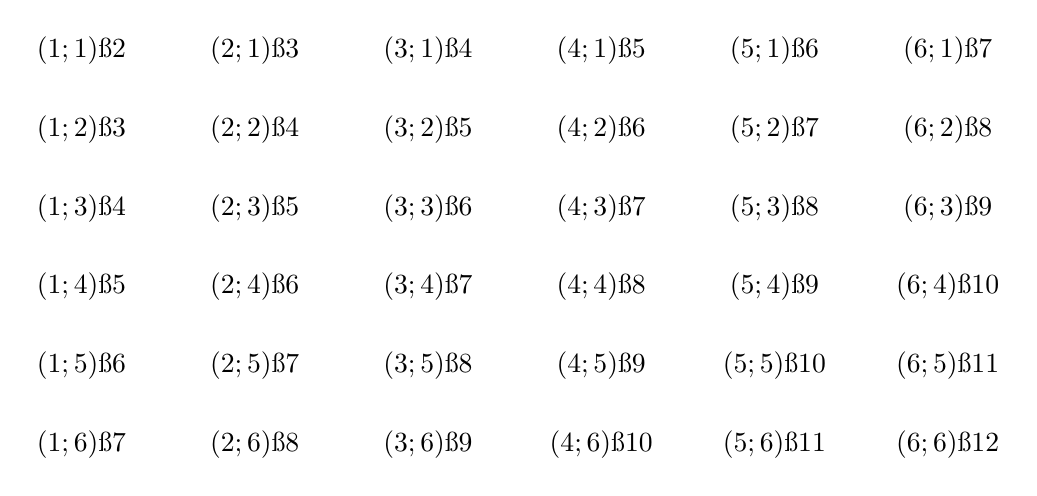
\begin{tikzpicture}
				      \node at (0,0) {$(1 ; 1) → 2$};
				      \node at (0,-1) {$(1 ; 2) → 3$};
				      \node at (0,-2) {$(1 ; 3) → 4$};
				      \foreach \y in {4,...,6} {
						      \node at (0,1-\y) {\correction{$(1 ; \y) → \pgfmathsetmacro\res{int(1+\y)}\res$}};
					      }
				      \foreach \x in {2,...,6} {
						      \foreach \y in {1,...,6} {
								      \node at (2.2*\x-2.2,1-\y) {\correction{$(\x ; \y) → \pgfmathsetmacro\res{int(\x+\y)}\res$}};
							      }
					      }
			      \end{tikzpicture}
		      \end{center}
		\item On admet que toutes les combinaisons listées ci-dessus ont la même chance d'être obtenues (on dit que la situation est \textbf{équiprobable}).

		      Quelle est alors la probabilité d'obtenir une combinaison particulière (par exemple $(4 ; 5)$) ?

		      \correction{Il y a $36$ combinaisons possibles, donc chaque combinaison à pour probabilité $\frac{1}{36}$.}
		\item En comptant le nombre de combinaisons dont la somme est $7$, déterminer la probabilité d'obtenir le résultat $7$.

		      \correction{$6$ combinaisons différentes donnent $7$, donc la probabilité est de $\frac{1}{36} = \frac{1}{6}$}
	\end{enumerate}
}

\Activite

\ifdefined\makeCorrection
\else
	\newpage\Activite
\fi

\end{document}